\documentclass{slide}

\title{Layered Architecture}
\subtitle{CSSE6400}
\author{Richard Thomas}
\date{\week{1}}

\usepackage{languages}
\usepackage{changepage}

\usepackage{tikz}
\usetikzlibrary{positioning}
\usetikzlibrary{fit}
\usetikzlibrary{arrows.meta}

\begin{document}

\maketitle

\quote[Shrek]{Ogres are like onions.\\
\highlight{Orgres have layers}, onions have layers...\\
You get it? We both have layers.}

\point[In the beginning...]{There was the big ball of mud \cite{ballofmud}}


\begin{frame}

\begin{figure}
    \href{https://tech.zensurance.com/posts/spaghetti-code}{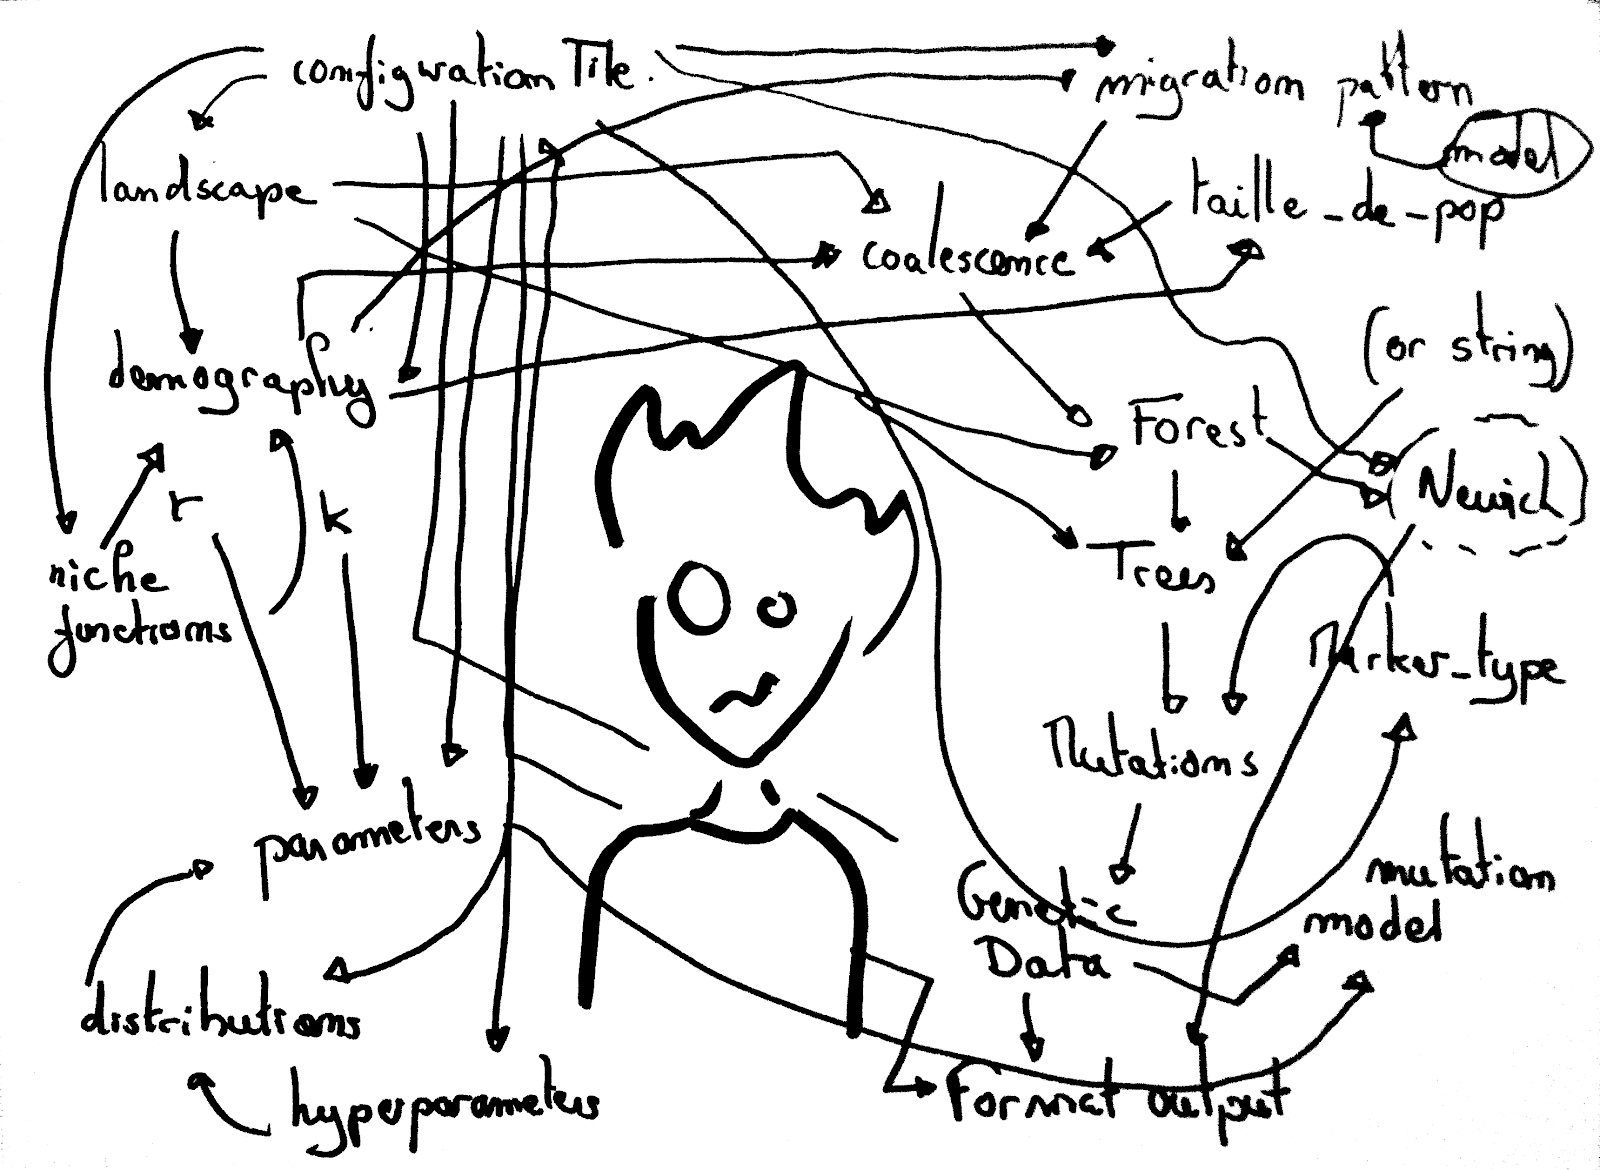
\includegraphics[height=\paperheight-11mm]{images/spaghetti-code.png}}
    \caption{Image from \href{https://tech.zensurance.com/posts/spaghetti-code}{``How to Avoid Spaghetti Code''} \cite{spaghetti-code}.}
\end{figure}

\end{frame}


\point[Problem]{Any change can affect any other part of the software.}

\point[``Solution'']{Layered architecture}


\begin{frame}
\begin{figure}[h]
    \centering
    \begin{tikzpicture}[component/.style={draw, anchor=center, text width=120pt}]
        \node [component](P) at (0,0)  {{\only<2>{\color{focus}} Presentation} Layer};
        \node [component] at (0,-1)  {{\only<3>{\color{focus}} Business} Layer};
        \node [component] at (0,-2)  {{\only<4>{\color{focus}} Persistence} Layer};
        \node [component](D) at (0,-3)  {{\only<5>{\color{focus}} Database} Layer};
    
        \node[draw, fit=(P) (D)](hardware) {};
    \end{tikzpicture}
    \caption{\highlight{Traditional} 4-tier, layered architecture.}
    \label{fig:traditional-layered}
\end{figure}
\end{frame}


\questionanswer{Can you identify an example of layered architecture?}{Pick any website.}


\begin{frame}

\begin{figure}
    \begin{adjustwidth}{-7mm}{-7mm}
        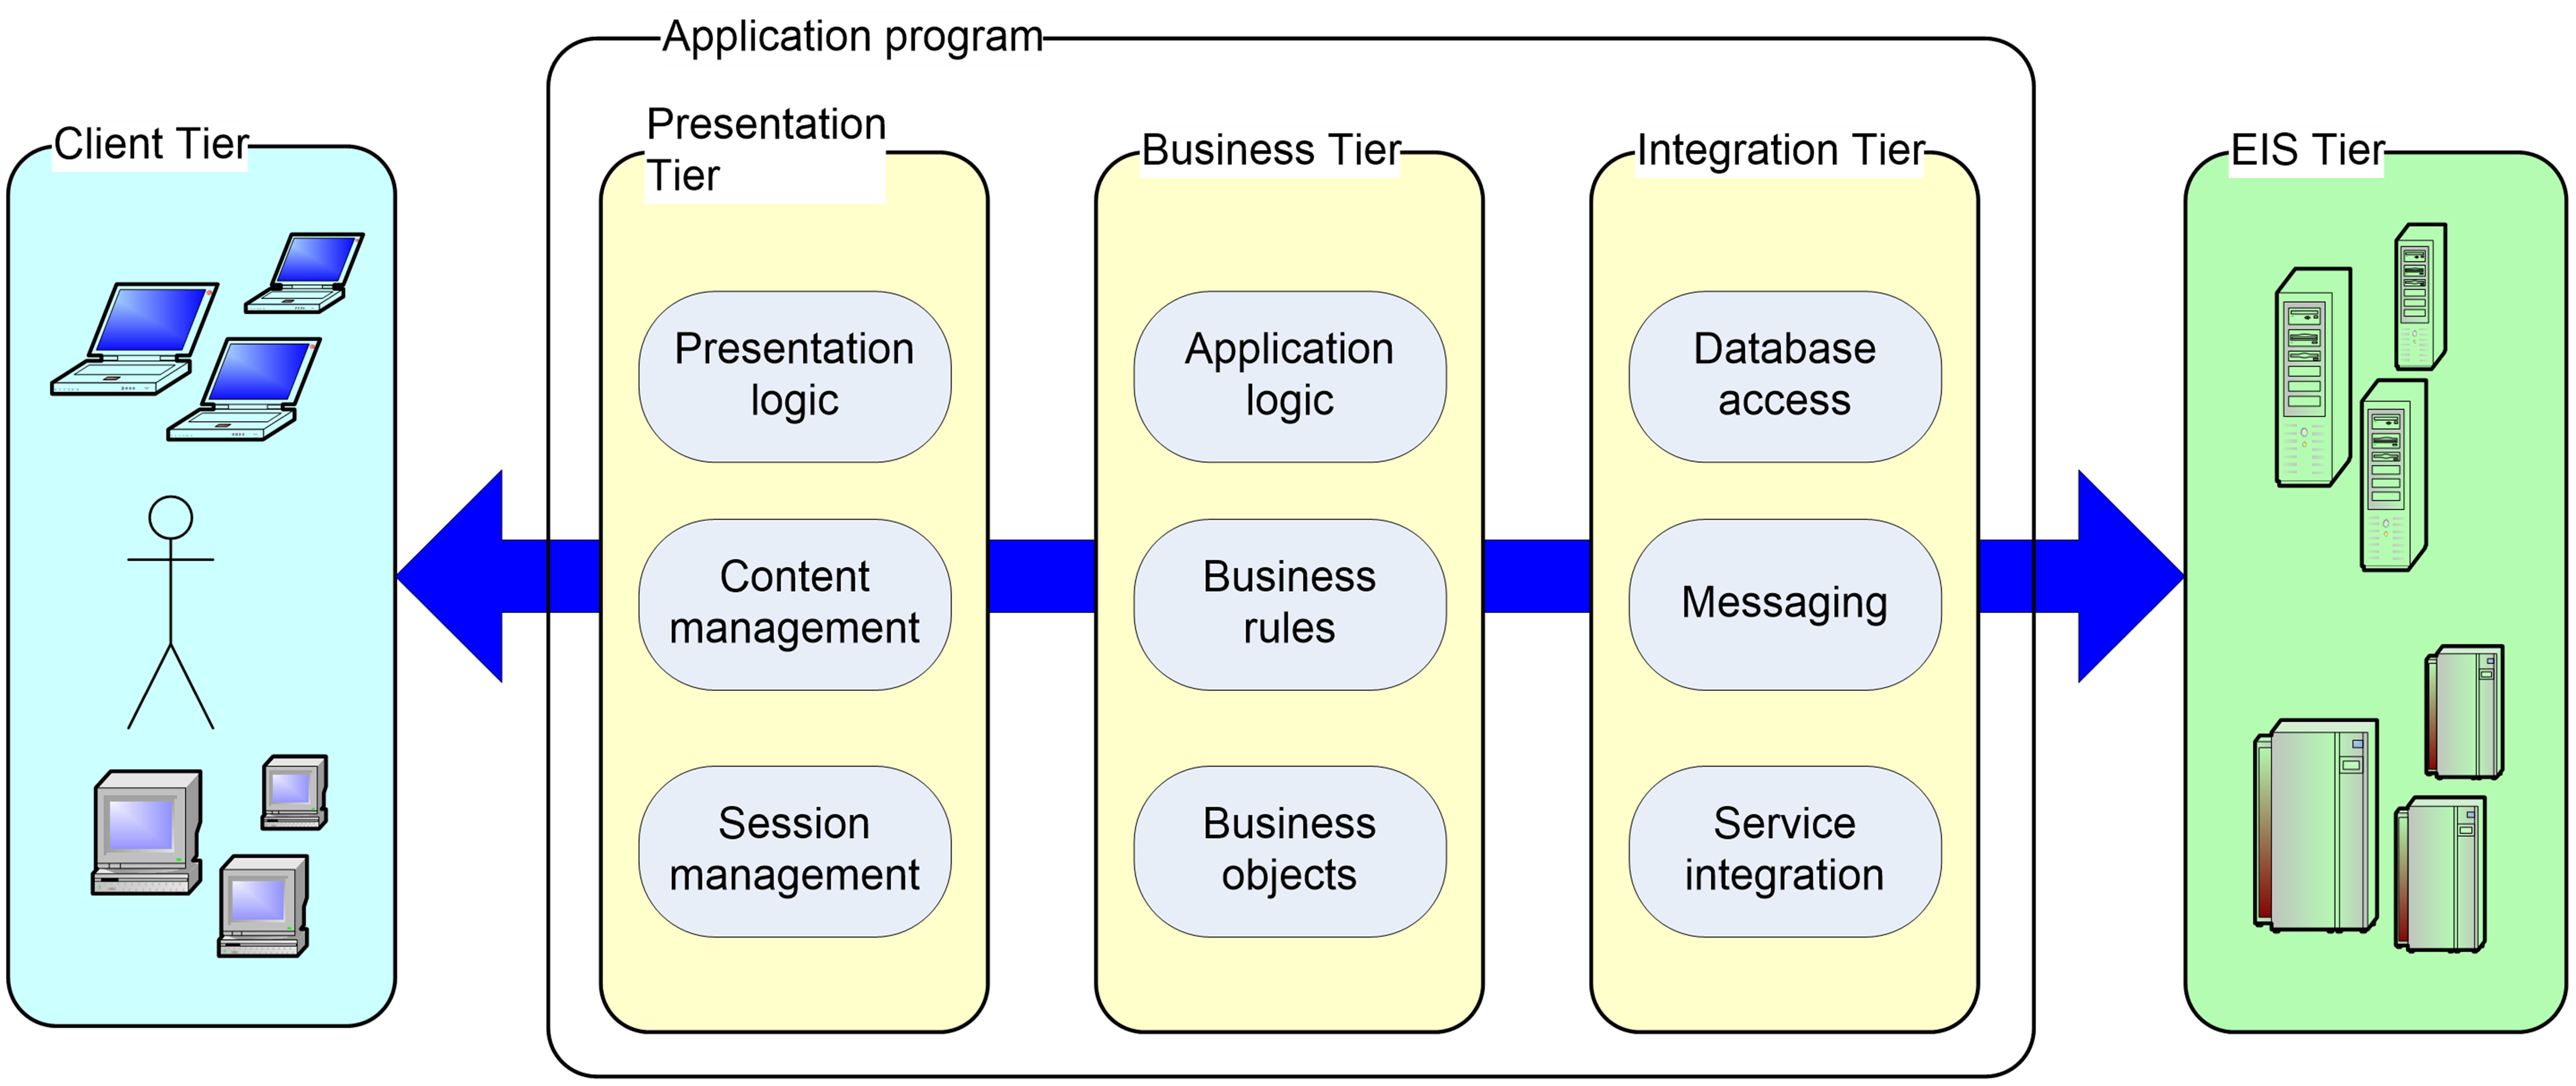
\includegraphics[width=0.96\paperwidth]{images/j2ee-arch.png}
    \end{adjustwidth}
    \caption{J2EE layered architecture (from \textit{Requirements Analysis and System Design} \cite{rasd2007}).}
\end{figure}

\end{frame}


\begin{frame}

\begin{figure}
    \centering
    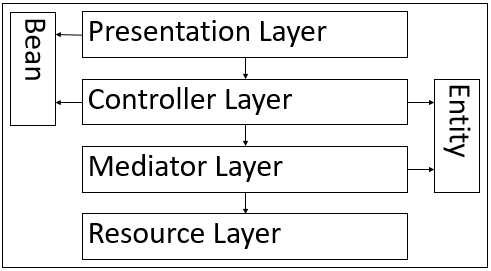
\includegraphics[width=0.5\paperwidth]{images/pcbmer.png}
    \caption{PCBMER layered architecture with sidecars (adapted from \textit{Requirements Analysis and System Design} \cite{rasd2007}).}
\end{figure}

\end{frame}


\begin{frame}{PCBMER Layers}

\large{
\begin{description}[<+->]
    \item[Presentation] Displays bean data, implements UI logic, and updates beans.
    \item[Controller] Implements application specific logic and instantiates beans.
    \item[Bean] Data transfer objects used by the Presentation layer.
    \item[Mediator] Manages business transactions, enforces business rules, instantiates business objects in the Entity layer, and manages the entity memory cache.
    \item[Entity] Classes representing persistent business objects.
    \item[Resource] Manages interactions with external persistent data sources.
\end{description}
}

\end{frame}


\definition{Layer Isolation Principle}
{Layers should not depend on implementation details of another layer.
Layers should only communicate through well defined interfaces (\emph{contracts}).}

\definition{Neighbour Communication Principle}
{Components can communicate across layers only through directly neighbouring layers.}

\definition{Downward Dependency Principle}
{Higher-level layers depend on lower layers, but lower-level layers are not dependent on higher layers.}

\definition{Upward Notification Principle}
{Lower layers communicate with higher layers using general interfaces, callbacks and/or events.
Dependencies are minimised by not relying on specific details published in a higher layer’s interface.}

\definition{Sidecar Spanning Principle}
{A sidecar layer contains interfaces that support complex communication between layers
(e.g. design patterns like the observer pattern) or external services (e.g. a logging framework).}

\point[Good architectural design...]{Applies these principles to deliver simple, modular designs that support modifiability.}


\references{articles,books}

\end{document}